\documentclass[twoside]{book}

% Packages required by doxygen
\usepackage{fixltx2e}
\usepackage{calc}
\usepackage{doxygen}
\usepackage[export]{adjustbox} % also loads graphicx
\usepackage{graphicx}
\usepackage[utf8]{inputenc}
\usepackage{makeidx}
\usepackage{multicol}
\usepackage{multirow}
\PassOptionsToPackage{warn}{textcomp}
\usepackage{textcomp}
\usepackage[nointegrals]{wasysym}
\usepackage[table]{xcolor}

% NLS support packages
\usepackage[french]{babel}

% Font selection
\usepackage[T1]{fontenc}
\usepackage[scaled=.90]{helvet}
\usepackage{courier}
\usepackage{amssymb}
\usepackage{sectsty}
\renewcommand{\familydefault}{\sfdefault}
\allsectionsfont{%
  \fontseries{bc}\selectfont%
  \color{darkgray}%
}
\renewcommand{\DoxyLabelFont}{%
  \fontseries{bc}\selectfont%
  \color{darkgray}%
}
\newcommand{\+}{\discretionary{\mbox{\scriptsize$\hookleftarrow$}}{}{}}

% Page & text layout
\usepackage{geometry}
\geometry{%
  a4paper,%
  top=2.5cm,%
  bottom=2.5cm,%
  left=2.5cm,%
  right=2.5cm%
}
\tolerance=750
\hfuzz=15pt
\hbadness=750
\setlength{\emergencystretch}{15pt}
\setlength{\parindent}{0cm}
\setlength{\parskip}{3ex plus 2ex minus 2ex}
\makeatletter
\renewcommand{\paragraph}{%
  \@startsection{paragraph}{4}{0ex}{-1.0ex}{1.0ex}{%
    \normalfont\normalsize\bfseries\SS@parafont%
  }%
}
\renewcommand{\subparagraph}{%
  \@startsection{subparagraph}{5}{0ex}{-1.0ex}{1.0ex}{%
    \normalfont\normalsize\bfseries\SS@subparafont%
  }%
}
\makeatother

% Headers & footers
\usepackage{fancyhdr}
\pagestyle{fancyplain}
\fancyhead[LE]{\fancyplain{}{\bfseries\thepage}}
\fancyhead[CE]{\fancyplain{}{}}
\fancyhead[RE]{\fancyplain{}{\bfseries\leftmark}}
\fancyhead[LO]{\fancyplain{}{\bfseries\rightmark}}
\fancyhead[CO]{\fancyplain{}{}}
\fancyhead[RO]{\fancyplain{}{\bfseries\thepage}}
\fancyfoot[LE]{\fancyplain{}{}}
\fancyfoot[CE]{\fancyplain{}{}}
\fancyfoot[RE]{\fancyplain{}{\bfseries\scriptsize Généré par Doxygen }}
\fancyfoot[LO]{\fancyplain{}{\bfseries\scriptsize Généré par Doxygen }}
\fancyfoot[CO]{\fancyplain{}{}}
\fancyfoot[RO]{\fancyplain{}{}}
\renewcommand{\footrulewidth}{0.4pt}
\renewcommand{\chaptermark}[1]{%
  \markboth{#1}{}%
}
\renewcommand{\sectionmark}[1]{%
  \markright{\thesection\ #1}%
}

% Indices & bibliography
\usepackage{natbib}
\usepackage[titles]{tocloft}
\setcounter{tocdepth}{3}
\setcounter{secnumdepth}{5}
\makeindex

% Hyperlinks (required, but should be loaded last)
\usepackage{ifpdf}
\ifpdf
  \usepackage[pdftex,pagebackref=true]{hyperref}
\else
  \usepackage[ps2pdf,pagebackref=true]{hyperref}
\fi
\hypersetup{%
  colorlinks=true,%
  linkcolor=blue,%
  citecolor=blue,%
  unicode%
}

% Custom commands
\newcommand{\clearemptydoublepage}{%
  \newpage{\pagestyle{empty}\cleardoublepage}%
}

\usepackage{caption}
\captionsetup{labelsep=space,justification=centering,font={bf},singlelinecheck=off,skip=4pt,position=top}

%===== C O N T E N T S =====

\begin{document}

% Titlepage & ToC
\hypersetup{pageanchor=false,
             bookmarksnumbered=true,
             pdfencoding=unicode
            }
\pagenumbering{alph}
\begin{titlepage}
\vspace*{7cm}
\begin{center}%
{\Large T\+P3 }\\
\vspace*{1cm}
{\large Généré par Doxygen 1.8.13}\\
\end{center}
\end{titlepage}
\clearemptydoublepage
\pagenumbering{roman}
\tableofcontents
\clearemptydoublepage
\pagenumbering{arabic}
\hypersetup{pageanchor=true}

%--- Begin generated contents ---
\chapter{Index hiérarchique}
\section{Hiérarchie des classes}
Cette liste d\textquotesingle{}héritage est classée approximativement par ordre alphabétique \+:\begin{DoxyCompactList}
\item \contentsline{section}{Complex\+Vector$<$ T $>$}{\pageref{class_complex_vector}}{}
\item \contentsline{section}{Dvector}{\pageref{class_dvector}}{}
\item \contentsline{section}{Gerstner\+Wave}{\pageref{class_gerstner_wave}}{}
\item \contentsline{section}{Height}{\pageref{class_height}}{}
\item \contentsline{section}{Ocean}{\pageref{class_ocean}}{}
\item \contentsline{section}{Philips\+Wave}{\pageref{class_philips_wave}}{}
\item \contentsline{section}{Wave\+Model}{\pageref{class_wave_model}}{}
\begin{DoxyCompactList}
\item \contentsline{section}{Gerstner\+Wave\+Model}{\pageref{class_gerstner_wave_model}}{}
\item \contentsline{section}{Philips\+Wave\+Model}{\pageref{class_philips_wave_model}}{}
\end{DoxyCompactList}
\end{DoxyCompactList}

\chapter{Index des classes}
\section{Liste des classes}
Liste des classes, structures, unions et interfaces avec une brève description \+:\begin{DoxyCompactList}
\item\contentsline{section}{\hyperlink{class_dvector}{Dvector} }{\pageref{class_dvector}}{}
\end{DoxyCompactList}

\chapter{Index des fichiers}
\section{Liste des fichiers}
Liste de tous les fichiers documentés avec une brève description \+:\begin{DoxyCompactList}
\item\contentsline{section}{{\bfseries test.\+h} }{\pageref{test_8h}}{}
\item\contentsline{section}{src/\hyperlink{_dvector_8h}{Dvector.\+h} }{\pageref{_dvector_8h}}{}
\end{DoxyCompactList}

\chapter{Documentation des classes}
\hypertarget{class_dvector}{}\section{Référence de la classe Dvector}
\label{class_dvector}\index{Dvector@{Dvector}}
\subsection*{Fonctions membres publiques}
\begin{DoxyCompactItemize}
\item 
\mbox{\Hypertarget{class_dvector_adf0f620df0feef3311f7d198e649a298}\label{class_dvector_adf0f620df0feef3311f7d198e649a298}} 
\hyperlink{class_dvector_adf0f620df0feef3311f7d198e649a298}{Dvector} ()
\begin{DoxyCompactList}\small\item\em Constructeur par défault. \end{DoxyCompactList}\item 
\hyperlink{class_dvector_a8a4feb509178ccc26a7d3805548fab17}{Dvector} (int \hyperlink{class_dvector_adda9654f389de24c744e897e93f850fb}{size}, int value=0)
\item 
\hyperlink{class_dvector_aa3a4f95e9bfe8139537593f86640d3af}{Dvector} (\hyperlink{class_dvector}{Dvector} const \&vect)
\begin{DoxyCompactList}\small\item\em Constructeur par recopie. \end{DoxyCompactList}\item 
\mbox{\Hypertarget{class_dvector_a2f2c20eb463fe2fd695493b5d6871244}\label{class_dvector_a2f2c20eb463fe2fd695493b5d6871244}} 
\hyperlink{class_dvector_a2f2c20eb463fe2fd695493b5d6871244}{Dvector} (std\+::string fichier)
\begin{DoxyCompactList}\small\item\em Constructeur à partir d\textquotesingle{}un fichier. \end{DoxyCompactList}\item 
\mbox{\Hypertarget{class_dvector_af66e4bdf60171463c01eea1039eecdb1}\label{class_dvector_af66e4bdf60171463c01eea1039eecdb1}} 
void \hyperlink{class_dvector_af66e4bdf60171463c01eea1039eecdb1}{display} (std\+::ostream \&str)
\begin{DoxyCompactList}\small\item\em Destructeur Destructeur de la classe \hyperlink{class_dvector}{Dvector}. \end{DoxyCompactList}\item 
\mbox{\Hypertarget{class_dvector_adda9654f389de24c744e897e93f850fb}\label{class_dvector_adda9654f389de24c744e897e93f850fb}} 
int \hyperlink{class_dvector_adda9654f389de24c744e897e93f850fb}{size} () const
\begin{DoxyCompactList}\small\item\em Taille du vecteur. \end{DoxyCompactList}\item 
void \hyperlink{class_dvector_a6fecdca0fbad7f928403597e322234b1}{fill\+Randomly} ()
\item 
\mbox{\Hypertarget{class_dvector_a2e07a00d750b98b10b3413227a7da46d}\label{class_dvector_a2e07a00d750b98b10b3413227a7da46d}} 
double \hyperlink{class_dvector_a2e07a00d750b98b10b3413227a7da46d}{get} (int index) const
\begin{DoxyCompactList}\small\item\em getter \end{DoxyCompactList}\item 
double \& \hyperlink{class_dvector_a237ba8b1ca7e68f78ec3f85ae800cbec}{operator()} (int i) const
\begin{DoxyCompactList}\small\item\em getter/setter \end{DoxyCompactList}\item 
void \hyperlink{class_dvector_a2ea1ba5bf87cebf7e74cb0dd94f90e12}{set} (int index, double value)
\begin{DoxyCompactList}\small\item\em setter \end{DoxyCompactList}\item 
void \hyperlink{class_dvector_a5d4b7a3273803031a7fb2b5516e5dd11}{set\+\_\+size} (int \hyperlink{class_dvector_adda9654f389de24c744e897e93f850fb}{size})
\begin{DoxyCompactList}\small\item\em changer la taille \end{DoxyCompactList}\item 
void \hyperlink{class_dvector_a99c6f3bc6f2d285ec2f9d8bd32a32218}{set\+\_\+v} (double $\ast$vect)
\begin{DoxyCompactList}\small\item\em changer tout les éléments du vecteurs \end{DoxyCompactList}\item 
\mbox{\Hypertarget{class_dvector_a100044e17131842814e0dee6c17e1ef7}\label{class_dvector_a100044e17131842814e0dee6c17e1ef7}} 
double $\ast$ \hyperlink{class_dvector_a100044e17131842814e0dee6c17e1ef7}{get\+\_\+v} () const
\begin{DoxyCompactList}\small\item\em getter de l\textquotesingle{}ensemble des éléments \end{DoxyCompactList}\item 
\mbox{\Hypertarget{class_dvector_a8f274704d0c2ffe625a9f56d5729158b}\label{class_dvector_a8f274704d0c2ffe625a9f56d5729158b}} 
\hyperlink{class_dvector}{Dvector} \hyperlink{class_dvector_a8f274704d0c2ffe625a9f56d5729158b}{get\+\_\+even} () const
\begin{DoxyCompactList}\small\item\em renvoie les composantes d\textquotesingle{}index pair \end{DoxyCompactList}\item 
\mbox{\Hypertarget{class_dvector_a190c6403a5318451b23ee276581c2618}\label{class_dvector_a190c6403a5318451b23ee276581c2618}} 
\hyperlink{class_dvector}{Dvector} \hyperlink{class_dvector_a190c6403a5318451b23ee276581c2618}{get\+\_\+odd} () const
\begin{DoxyCompactList}\small\item\em renvoie les composantes d\textquotesingle{}index impair \end{DoxyCompactList}\item 
\mbox{\Hypertarget{class_dvector_a9c72bc1fb55c36844d55b996127e7be7}\label{class_dvector_a9c72bc1fb55c36844d55b996127e7be7}} 
\hyperlink{class_dvector}{Dvector} {\bfseries operator=} (const \hyperlink{class_dvector}{Dvector} \&vect)
\item 
\mbox{\Hypertarget{class_dvector_a75c5523da365463f4efa812a44596409}\label{class_dvector_a75c5523da365463f4efa812a44596409}} 
\hyperlink{class_dvector}{Dvector} {\bfseries operator+=} (const \hyperlink{class_dvector}{Dvector} \&vect)
\item 
\mbox{\Hypertarget{class_dvector_a472907173bf8eaf0aaa0ff9bde8f125e}\label{class_dvector_a472907173bf8eaf0aaa0ff9bde8f125e}} 
\hyperlink{class_dvector}{Dvector} {\bfseries operator-\/=} (const \hyperlink{class_dvector}{Dvector} \&vect)
\item 
\mbox{\Hypertarget{class_dvector_af31badc85a41de4257f0b2a870c5cc84}\label{class_dvector_af31badc85a41de4257f0b2a870c5cc84}} 
\hyperlink{class_dvector}{Dvector} {\bfseries operator$\ast$=} (int i)
\item 
\mbox{\Hypertarget{class_dvector_ad4ead0c93b44fc1d1b31e58d4f7e0a78}\label{class_dvector_ad4ead0c93b44fc1d1b31e58d4f7e0a78}} 
\hyperlink{class_dvector}{Dvector} {\bfseries operator$\ast$=} (const \hyperlink{class_dvector}{Dvector} \&vect)
\item 
\mbox{\Hypertarget{class_dvector_a184af91c3a82d4225382e3bc2f21f21c}\label{class_dvector_a184af91c3a82d4225382e3bc2f21f21c}} 
\hyperlink{class_dvector}{Dvector} {\bfseries operator/=} (int i)
\item 
\mbox{\Hypertarget{class_dvector_aabff73704ce72471069bc304bd6e6ca5}\label{class_dvector_aabff73704ce72471069bc304bd6e6ca5}} 
\hyperlink{class_dvector}{Dvector} {\bfseries operator+} (int i)
\item 
\mbox{\Hypertarget{class_dvector_a801899c54a142444de7156e718ef559b}\label{class_dvector_a801899c54a142444de7156e718ef559b}} 
\hyperlink{class_dvector}{Dvector} {\bfseries operator-\/} (int i)
\item 
\mbox{\Hypertarget{class_dvector_a2bd2d56073f1dfe48c8387537c51c882}\label{class_dvector_a2bd2d56073f1dfe48c8387537c51c882}} 
\hyperlink{class_dvector}{Dvector} {\bfseries operator$\ast$} (int i)
\item 
\mbox{\Hypertarget{class_dvector_abe59641937a4b5222445c3df1618ee2c}\label{class_dvector_abe59641937a4b5222445c3df1618ee2c}} 
double {\bfseries operator$\ast$} (const \hyperlink{class_dvector}{Dvector} \&vect)
\item 
\mbox{\Hypertarget{class_dvector_a281d788b6a6c1c7b076684c20f63210f}\label{class_dvector_a281d788b6a6c1c7b076684c20f63210f}} 
\hyperlink{class_dvector}{Dvector} {\bfseries operator/} (int i)
\item 
\mbox{\Hypertarget{class_dvector_ad6d5934a4a49287611e35fc1bdd8d357}\label{class_dvector_ad6d5934a4a49287611e35fc1bdd8d357}} 
\hyperlink{class_dvector}{Dvector} {\bfseries operator+} (\hyperlink{class_dvector}{Dvector} \&vect)
\item 
\mbox{\Hypertarget{class_dvector_a27515c1928c6602c0b8b5a9c5a7dfffe}\label{class_dvector_a27515c1928c6602c0b8b5a9c5a7dfffe}} 
\hyperlink{class_dvector}{Dvector} {\bfseries operator-\/} (\hyperlink{class_dvector}{Dvector} \&vect)
\item 
\mbox{\Hypertarget{class_dvector_a402617afbca77199f537110a8efc0e10}\label{class_dvector_a402617afbca77199f537110a8efc0e10}} 
\hyperlink{class_dvector}{Dvector} {\bfseries operator-\/} ()
\item 
\mbox{\Hypertarget{class_dvector_ae124565a643023393c191cc0acaa44b5}\label{class_dvector_ae124565a643023393c191cc0acaa44b5}} 
bool {\bfseries operator==} (const \hyperlink{class_dvector}{Dvector} \&vect)
\item 
void \hyperlink{class_dvector_a3df83649e0ed9cf7c21fe03fdef8b2f4}{resize} (int \hyperlink{class_dvector_adda9654f389de24c744e897e93f850fb}{size}, double $\ast$vect=0)
\begin{DoxyCompactList}\small\item\em Changer la taille et insérer de nouvelles valeurs en queue. \end{DoxyCompactList}\item 
\mbox{\Hypertarget{class_dvector_a2300bc9dff4d2bf480a22bf88c37085b}\label{class_dvector_a2300bc9dff4d2bf480a22bf88c37085b}} 
bool \hyperlink{class_dvector_a2300bc9dff4d2bf480a22bf88c37085b}{isnull} ()
\begin{DoxyCompactList}\small\item\em Verification de nullitude. \end{DoxyCompactList}\end{DoxyCompactItemize}


\subsection{Documentation des constructeurs et destructeur}
\mbox{\Hypertarget{class_dvector_a8a4feb509178ccc26a7d3805548fab17}\label{class_dvector_a8a4feb509178ccc26a7d3805548fab17}} 
\index{Dvector@{Dvector}!Dvector@{Dvector}}
\index{Dvector@{Dvector}!Dvector@{Dvector}}
\subsubsection{\texorpdfstring{Dvector()}{Dvector()}\hspace{0.1cm}{\footnotesize\ttfamily [1/2]}}
{\footnotesize\ttfamily Dvector\+::\+Dvector (\begin{DoxyParamCaption}\item[{int}]{size,  }\item[{int}]{value = {\ttfamily 0} }\end{DoxyParamCaption})}

Constructeur avec remplissage à valeur fixe 
\begin{DoxyParams}{Paramètres}
{\em size} & \+: taille du vecteur \\
\hline
{\em value} & \+: la valeur à mettre dans toutes les cases \\
\hline
\end{DoxyParams}
\mbox{\Hypertarget{class_dvector_aa3a4f95e9bfe8139537593f86640d3af}\label{class_dvector_aa3a4f95e9bfe8139537593f86640d3af}} 
\index{Dvector@{Dvector}!Dvector@{Dvector}}
\index{Dvector@{Dvector}!Dvector@{Dvector}}
\subsubsection{\texorpdfstring{Dvector()}{Dvector()}\hspace{0.1cm}{\footnotesize\ttfamily [2/2]}}
{\footnotesize\ttfamily Dvector\+::\+Dvector (\begin{DoxyParamCaption}\item[{\hyperlink{class_dvector}{Dvector} const \&}]{vect }\end{DoxyParamCaption})}



Constructeur par recopie. 


\begin{DoxyParams}{Paramètres}
{\em vect} & \+: le vecteur à recopier \\
\hline
\end{DoxyParams}


\subsection{Documentation des fonctions membres}
\mbox{\Hypertarget{class_dvector_a6fecdca0fbad7f928403597e322234b1}\label{class_dvector_a6fecdca0fbad7f928403597e322234b1}} 
\index{Dvector@{Dvector}!fill\+Randomly@{fill\+Randomly}}
\index{fill\+Randomly@{fill\+Randomly}!Dvector@{Dvector}}
\subsubsection{\texorpdfstring{fill\+Randomly()}{fillRandomly()}}
{\footnotesize\ttfamily void Dvector\+::fill\+Randomly (\begin{DoxyParamCaption}{ }\end{DoxyParamCaption})}

Remplit le vecteur de manière aléatoire \mbox{\Hypertarget{class_dvector_a237ba8b1ca7e68f78ec3f85ae800cbec}\label{class_dvector_a237ba8b1ca7e68f78ec3f85ae800cbec}} 
\index{Dvector@{Dvector}!operator()@{operator()}}
\index{operator()@{operator()}!Dvector@{Dvector}}
\subsubsection{\texorpdfstring{operator()()}{operator()()}}
{\footnotesize\ttfamily double \& Dvector\+::operator() (\begin{DoxyParamCaption}\item[{int}]{i }\end{DoxyParamCaption}) const}



getter/setter 


\begin{DoxyParams}{Paramètres}
{\em i} & \+: index \\
\hline
\end{DoxyParams}
\mbox{\Hypertarget{class_dvector_a3df83649e0ed9cf7c21fe03fdef8b2f4}\label{class_dvector_a3df83649e0ed9cf7c21fe03fdef8b2f4}} 
\index{Dvector@{Dvector}!resize@{resize}}
\index{resize@{resize}!Dvector@{Dvector}}
\subsubsection{\texorpdfstring{resize()}{resize()}}
{\footnotesize\ttfamily void Dvector\+::resize (\begin{DoxyParamCaption}\item[{int}]{size,  }\item[{double $\ast$}]{vect = {\ttfamily 0} }\end{DoxyParamCaption})}



Changer la taille et insérer de nouvelles valeurs en queue. 


\begin{DoxyParams}{Paramètres}
{\em size} & \+: la nouvelle taille du vecteur \\
\hline
{\em vect} & \+: le vecteur de valeurs à insérer en queue si la nouvelle taille est supérieure à l\textquotesingle{}ancienne \\
\hline
\end{DoxyParams}
\mbox{\Hypertarget{class_dvector_a2ea1ba5bf87cebf7e74cb0dd94f90e12}\label{class_dvector_a2ea1ba5bf87cebf7e74cb0dd94f90e12}} 
\index{Dvector@{Dvector}!set@{set}}
\index{set@{set}!Dvector@{Dvector}}
\subsubsection{\texorpdfstring{set()}{set()}}
{\footnotesize\ttfamily void Dvector\+::set (\begin{DoxyParamCaption}\item[{int}]{index,  }\item[{double}]{value }\end{DoxyParamCaption})}



setter 


\begin{DoxyParams}{Paramètres}
{\em index} & \+: index de l\textquotesingle{}élément à modifier \\
\hline
{\em value} & \+: la valeur à insérer \\
\hline
\end{DoxyParams}
\mbox{\Hypertarget{class_dvector_a5d4b7a3273803031a7fb2b5516e5dd11}\label{class_dvector_a5d4b7a3273803031a7fb2b5516e5dd11}} 
\index{Dvector@{Dvector}!set\+\_\+size@{set\+\_\+size}}
\index{set\+\_\+size@{set\+\_\+size}!Dvector@{Dvector}}
\subsubsection{\texorpdfstring{set\+\_\+size()}{set\_size()}}
{\footnotesize\ttfamily void Dvector\+::set\+\_\+size (\begin{DoxyParamCaption}\item[{int}]{size }\end{DoxyParamCaption})}



changer la taille 


\begin{DoxyParams}{Paramètres}
{\em size} & \+: la nouvelle taille \\
\hline
\end{DoxyParams}
\mbox{\Hypertarget{class_dvector_a99c6f3bc6f2d285ec2f9d8bd32a32218}\label{class_dvector_a99c6f3bc6f2d285ec2f9d8bd32a32218}} 
\index{Dvector@{Dvector}!set\+\_\+v@{set\+\_\+v}}
\index{set\+\_\+v@{set\+\_\+v}!Dvector@{Dvector}}
\subsubsection{\texorpdfstring{set\+\_\+v()}{set\_v()}}
{\footnotesize\ttfamily void Dvector\+::set\+\_\+v (\begin{DoxyParamCaption}\item[{double $\ast$}]{vect }\end{DoxyParamCaption})}



changer tout les éléments du vecteurs 


\begin{DoxyParams}{Paramètres}
{\em $\ast$vect} & \+: pointeur des nouveaux éléments \\
\hline
\end{DoxyParams}


La documentation de cette classe a été générée à partir des fichiers suivants \+:\begin{DoxyCompactItemize}
\item 
/home/louis/\+Documents/2\+A/\+M\+P\+C/\+C\+P\+P/\+T\+P4\+\_\+sonoleta/headers/\hyperlink{_dvector_8h}{Dvector.\+h}\item 
/home/louis/\+Documents/2\+A/\+M\+P\+C/\+C\+P\+P/\+T\+P4\+\_\+sonoleta/src/Dvector.\+cpp\end{DoxyCompactItemize}

\hypertarget{class_gerstner_wave}{}\section{Référence de la classe Gerstner\+Wave}
\label{class_gerstner_wave}\index{Gerstner\+Wave@{Gerstner\+Wave}}
\subsection*{Fonctions membres publiques}
\begin{DoxyCompactItemize}
\item 
\mbox{\Hypertarget{class_gerstner_wave_a207ffe78993b42001d763a0e39b99f07}\label{class_gerstner_wave_a207ffe78993b42001d763a0e39b99f07}} 
\hyperlink{class_gerstner_wave_a207ffe78993b42001d763a0e39b99f07}{Gerstner\+Wave} ()
\begin{DoxyCompactList}\small\item\em Constructeur par défaut. \end{DoxyCompactList}\item 
\mbox{\Hypertarget{class_gerstner_wave_af3df02ad2ba5fa164c83e332eabadfea}\label{class_gerstner_wave_af3df02ad2ba5fa164c83e332eabadfea}} 
\hyperlink{class_gerstner_wave_af3df02ad2ba5fa164c83e332eabadfea}{$\sim$\+Gerstner\+Wave} ()
\begin{DoxyCompactList}\small\item\em Destructeur Destructeur de la classe \hyperlink{class_dvector}{Dvector}. \end{DoxyCompactList}\item 
\hyperlink{class_gerstner_wave_aca3a91ab8ae49e3814bfd5b6e4607f31}{Gerstner\+Wave} (double A, double Phi, \hyperlink{class_dvector}{Dvector} $\ast$dir, double freq)
\item 
\mbox{\Hypertarget{class_gerstner_wave_a5e019cb6bf88fae82be53dcbfb2c5109}\label{class_gerstner_wave_a5e019cb6bf88fae82be53dcbfb2c5109}} 
{\bfseries Gerstner\+Wave} (\hyperlink{class_gerstner_wave}{Gerstner\+Wave} \&\&model)
\item 
\mbox{\Hypertarget{class_gerstner_wave_aba4dcf8262af3cbc677804c63f9104d4}\label{class_gerstner_wave_aba4dcf8262af3cbc677804c63f9104d4}} 
{\bfseries Gerstner\+Wave} (\hyperlink{class_gerstner_wave}{Gerstner\+Wave} const \&model)
\item 
\mbox{\Hypertarget{class_gerstner_wave_aa2773b91856128983df03e8983970e86}\label{class_gerstner_wave_aa2773b91856128983df03e8983970e86}} 
\hyperlink{class_gerstner_wave}{Gerstner\+Wave} {\bfseries operator=} (\hyperlink{class_gerstner_wave}{Gerstner\+Wave} \&\&model)
\item 
\mbox{\Hypertarget{class_gerstner_wave_ae776ca443eb1bf78bcb296686ccf27ae}\label{class_gerstner_wave_ae776ca443eb1bf78bcb296686ccf27ae}} 
\hyperlink{class_gerstner_wave}{Gerstner\+Wave} {\bfseries operator=} (\hyperlink{class_gerstner_wave}{Gerstner\+Wave} const \&model)
\item 
\mbox{\Hypertarget{class_gerstner_wave_aef62ae747a5a0224e026df4441cfb857}\label{class_gerstner_wave_aef62ae747a5a0224e026df4441cfb857}} 
double {\bfseries operator()} (\hyperlink{class_dvector}{Dvector} x0, int t)
\item 
\mbox{\Hypertarget{class_gerstner_wave_a4b3989096ad666a3daf18c9e61a33818}\label{class_gerstner_wave_a4b3989096ad666a3daf18c9e61a33818}} 
double {\bfseries get\+Amplitude} ()
\item 
\mbox{\Hypertarget{class_gerstner_wave_a3b499d792884b962fadfd58b3003c2c2}\label{class_gerstner_wave_a3b499d792884b962fadfd58b3003c2c2}} 
void {\bfseries set\+Amplitude} (double value)
\item 
\mbox{\Hypertarget{class_gerstner_wave_aec45e17327906cf1aa7e746a5cd92596}\label{class_gerstner_wave_aec45e17327906cf1aa7e746a5cd92596}} 
double {\bfseries get\+Phase} ()
\item 
\mbox{\Hypertarget{class_gerstner_wave_a4e5a1f7f408d79bb2eab24cdfa5cdf08}\label{class_gerstner_wave_a4e5a1f7f408d79bb2eab24cdfa5cdf08}} 
void {\bfseries set\+Phase} (double value)
\item 
\mbox{\Hypertarget{class_gerstner_wave_ade0e4f9a29e27253a7096cf37dcd52d6}\label{class_gerstner_wave_ade0e4f9a29e27253a7096cf37dcd52d6}} 
\hyperlink{class_dvector}{Dvector} $\ast$ {\bfseries get\+Direction} ()
\item 
\mbox{\Hypertarget{class_gerstner_wave_a722535521e43ba6f6c5e28a578ee824b}\label{class_gerstner_wave_a722535521e43ba6f6c5e28a578ee824b}} 
void {\bfseries set\+Direction} (\hyperlink{class_dvector}{Dvector} $\ast$value)
\item 
\mbox{\Hypertarget{class_gerstner_wave_a254b842667e2a2c6ce10f0f7b965c458}\label{class_gerstner_wave_a254b842667e2a2c6ce10f0f7b965c458}} 
double {\bfseries get\+Frequency} ()
\item 
\mbox{\Hypertarget{class_gerstner_wave_a7ea4b613d091da359115183c43ddeb2a}\label{class_gerstner_wave_a7ea4b613d091da359115183c43ddeb2a}} 
void {\bfseries set\+Frequency} (double value)
\end{DoxyCompactItemize}


\subsection{Documentation des constructeurs et destructeur}
\mbox{\Hypertarget{class_gerstner_wave_aca3a91ab8ae49e3814bfd5b6e4607f31}\label{class_gerstner_wave_aca3a91ab8ae49e3814bfd5b6e4607f31}} 
\index{Gerstner\+Wave@{Gerstner\+Wave}!Gerstner\+Wave@{Gerstner\+Wave}}
\index{Gerstner\+Wave@{Gerstner\+Wave}!Gerstner\+Wave@{Gerstner\+Wave}}
\subsubsection{\texorpdfstring{Gerstner\+Wave()}{GerstnerWave()}}
{\footnotesize\ttfamily Gerstner\+Wave\+::\+Gerstner\+Wave (\begin{DoxyParamCaption}\item[{double}]{A,  }\item[{double}]{Phi,  }\item[{\hyperlink{class_dvector}{Dvector} $\ast$}]{dir,  }\item[{double}]{freq }\end{DoxyParamCaption})}

Constructeur 
\begin{DoxyParams}{Paramètres}
{\em A} & \+: amplitude de l\textquotesingle{}onde \\
\hline
{\em Phi} & \+: phase de l\textquotesingle{}onde \\
\hline
{\em $\ast$dir} & \+: direction du vecteur d\textquotesingle{}onde \\
\hline
{\em freq} & \+: frequence de l\textquotesingle{}onde \\
\hline
\end{DoxyParams}


La documentation de cette classe a été générée à partir des fichiers suivants \+:\begin{DoxyCompactItemize}
\item 
/home/louis/\+Documents/2\+A/\+M\+P\+C/\+C\+P\+P/\+T\+P3\+\_\+sonoleta/headers/\hyperlink{_gerstner_wave_8h}{Gerstner\+Wave.\+h}\item 
/home/louis/\+Documents/2\+A/\+M\+P\+C/\+C\+P\+P/\+T\+P3\+\_\+sonoleta/src/Gerstner\+Wave.\+cpp\end{DoxyCompactItemize}

\hypertarget{class_gerstner_wave_model}{}\section{Référence de la classe Gerstner\+Wave\+Model}
\label{class_gerstner_wave_model}\index{Gerstner\+Wave\+Model@{Gerstner\+Wave\+Model}}


Graphe d\textquotesingle{}héritage de Gerstner\+Wave\+Model\+:
\nopagebreak
\begin{figure}[H]
\begin{center}
\leavevmode
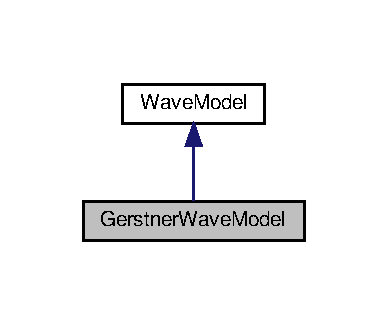
\includegraphics[width=186pt]{class_gerstner_wave_model__inherit__graph}
\end{center}
\end{figure}


Graphe de collaboration de Gerstner\+Wave\+Model\+:
\nopagebreak
\begin{figure}[H]
\begin{center}
\leavevmode
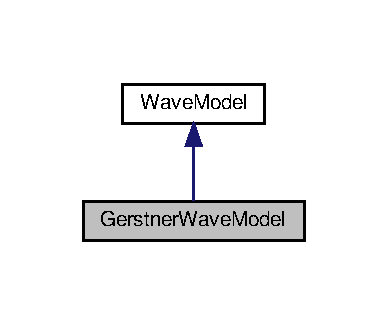
\includegraphics[width=186pt]{class_gerstner_wave_model__coll__graph}
\end{center}
\end{figure}
\subsection*{Fonctions membres publiques}
\begin{DoxyCompactItemize}
\item 
\mbox{\Hypertarget{class_gerstner_wave_model_ab600b7a3f7455d94ff0069fa47b355bc}\label{class_gerstner_wave_model_ab600b7a3f7455d94ff0069fa47b355bc}} 
{\bfseries Gerstner\+Wave\+Model} (int n)
\item 
\mbox{\Hypertarget{class_gerstner_wave_model_adc09d3aaaee69d0e66d776d93c807d37}\label{class_gerstner_wave_model_adc09d3aaaee69d0e66d776d93c807d37}} 
{\bfseries Gerstner\+Wave\+Model} (\hyperlink{class_gerstner_wave_model}{Gerstner\+Wave\+Model} \&\&model)
\item 
\mbox{\Hypertarget{class_gerstner_wave_model_afa36f5bb46de8f5be4b12d2b4e22cefb}\label{class_gerstner_wave_model_afa36f5bb46de8f5be4b12d2b4e22cefb}} 
{\bfseries Gerstner\+Wave\+Model} (\hyperlink{class_gerstner_wave_model}{Gerstner\+Wave\+Model} const \&model)
\item 
\mbox{\Hypertarget{class_gerstner_wave_model_a368e6ba6e59bb5ae666ddd3b11166f49}\label{class_gerstner_wave_model_a368e6ba6e59bb5ae666ddd3b11166f49}} 
\hyperlink{class_gerstner_wave_model}{Gerstner\+Wave\+Model} \& {\bfseries operator=} (\hyperlink{class_gerstner_wave_model}{Gerstner\+Wave\+Model} \&\&model)
\item 
\mbox{\Hypertarget{class_gerstner_wave_model_ae57c58cad23189d3ddb97d7520c01341}\label{class_gerstner_wave_model_ae57c58cad23189d3ddb97d7520c01341}} 
\hyperlink{class_gerstner_wave_model}{Gerstner\+Wave\+Model} \& {\bfseries operator=} (\hyperlink{class_gerstner_wave_model}{Gerstner\+Wave\+Model} const \&model)
\item 
\mbox{\Hypertarget{class_gerstner_wave_model_ac984a0700f00aac266b97973cc13b636}\label{class_gerstner_wave_model_ac984a0700f00aac266b97973cc13b636}} 
void {\bfseries set\+Gerstner\+Wave} (int i, \hyperlink{class_gerstner_wave}{Gerstner\+Wave} wave)
\end{DoxyCompactItemize}


La documentation de cette classe a été générée à partir des fichiers suivants \+:\begin{DoxyCompactItemize}
\item 
/home/louis/\+Documents/2\+A/\+M\+P\+C/\+C\+P\+P/\+T\+P3\+\_\+sonoleta/headers/\hyperlink{_gerstner_wave_model_8h}{Gerstner\+Wave\+Model.\+h}\item 
/home/louis/\+Documents/2\+A/\+M\+P\+C/\+C\+P\+P/\+T\+P3\+\_\+sonoleta/src/Gerstner\+Wave\+Model.\+cpp\end{DoxyCompactItemize}

\hypertarget{class_height}{}\section{Référence de la classe Height}
\label{class_height}\index{Height@{Height}}
\subsection*{Fonctions membres publiques}
\begin{DoxyCompactItemize}
\item 
\hyperlink{class_height_af4c985463352fc7f3dd6b00574ef865b}{Height} (int n\+\_\+x, int n\+\_\+y, double L\+\_\+x, double L\+\_\+y)
\begin{DoxyCompactList}\small\item\em Constructeur. \end{DoxyCompactList}\item 
\mbox{\Hypertarget{class_height_a39b74091414bcb55a3d9023cab5496f4}\label{class_height_a39b74091414bcb55a3d9023cab5496f4}} 
{\bfseries Height} (\hyperlink{class_height}{Height} \&\&hauteurs)
\item 
\mbox{\Hypertarget{class_height_a0d36a635165e5b77d0034aaef6b895dc}\label{class_height_a0d36a635165e5b77d0034aaef6b895dc}} 
{\bfseries Height} (\hyperlink{class_height}{Height} const \&hauteurs)
\item 
\mbox{\Hypertarget{class_height_aab8a602d0a015dba9526361a635cf912}\label{class_height_aab8a602d0a015dba9526361a635cf912}} 
\hyperlink{class_height}{Height} {\bfseries operator=} (\hyperlink{class_height}{Height} \&\&hauteurs)
\item 
\mbox{\Hypertarget{class_height_a1abcb7d9d453779226a2f211d4c1f5c5}\label{class_height_a1abcb7d9d453779226a2f211d4c1f5c5}} 
\hyperlink{class_height}{Height} {\bfseries operator=} (\hyperlink{class_height}{Height} const \&hauteurs)
\item 
\mbox{\Hypertarget{class_height_af946b05c8753d5240a7719d5716b851e}\label{class_height_af946b05c8753d5240a7719d5716b851e}} 
double {\bfseries operator()} (int x, int y)
\item 
\mbox{\Hypertarget{class_height_a4bac735463fe0500e533a651afacf19d}\label{class_height_a4bac735463fe0500e533a651afacf19d}} 
void {\bfseries set\+Lx} (double value)
\item 
\mbox{\Hypertarget{class_height_a8edebe5c97f6adb896865d46c1d355f6}\label{class_height_a8edebe5c97f6adb896865d46c1d355f6}} 
double {\bfseries get\+Lx} ()
\item 
\mbox{\Hypertarget{class_height_a2b324a15c13bcdaebea700937285becd}\label{class_height_a2b324a15c13bcdaebea700937285becd}} 
void {\bfseries set\+Ly} (double value)
\item 
\mbox{\Hypertarget{class_height_a837ec9f1c378eee4222c56045e5d1bfe}\label{class_height_a837ec9f1c378eee4222c56045e5d1bfe}} 
double {\bfseries get\+Ly} ()
\item 
\mbox{\Hypertarget{class_height_ad2be1933f92071caeb1d743239244fc4}\label{class_height_ad2be1933f92071caeb1d743239244fc4}} 
void {\bfseries set\+Nx} (int value)
\item 
\mbox{\Hypertarget{class_height_a3ff565c348e61bef5d2e22163666d6ca}\label{class_height_a3ff565c348e61bef5d2e22163666d6ca}} 
double {\bfseries get\+Nx} ()
\item 
\mbox{\Hypertarget{class_height_ab3bacc10cd3ae023dcc54c71f2f803fe}\label{class_height_ab3bacc10cd3ae023dcc54c71f2f803fe}} 
void {\bfseries set\+Ny} (int value)
\item 
\mbox{\Hypertarget{class_height_a3136f6b29a3318c8e8e160cd077e0f88}\label{class_height_a3136f6b29a3318c8e8e160cd077e0f88}} 
double {\bfseries get\+Ny} ()
\item 
\mbox{\Hypertarget{class_height_aff97482f65f6e17879620854a364151a}\label{class_height_aff97482f65f6e17879620854a364151a}} 
void {\bfseries set\+Value} (int x, int y, double value)
\item 
\mbox{\Hypertarget{class_height_a5d6efd53512f0771e157d36da0b41704}\label{class_height_a5d6efd53512f0771e157d36da0b41704}} 
void {\bfseries plot} (std\+::string path)
\end{DoxyCompactItemize}


\subsection{Documentation des constructeurs et destructeur}
\mbox{\Hypertarget{class_height_af4c985463352fc7f3dd6b00574ef865b}\label{class_height_af4c985463352fc7f3dd6b00574ef865b}} 
\index{Height@{Height}!Height@{Height}}
\index{Height@{Height}!Height@{Height}}
\subsubsection{\texorpdfstring{Height()}{Height()}}
{\footnotesize\ttfamily Height\+::\+Height (\begin{DoxyParamCaption}\item[{int}]{n\+\_\+x,  }\item[{int}]{n\+\_\+y,  }\item[{double}]{L\+\_\+x,  }\item[{double}]{L\+\_\+y }\end{DoxyParamCaption})}



Constructeur. 


\begin{DoxyParams}{Paramètres}
{\em n\+\_\+x} & \+: nombre de points de discrétisation selon x \\
\hline
{\em n\+\_\+y} & \+: nombre de points de discrétisation selon y \\
\hline
{\em L\+\_\+x} & \+: taille du domaine selon x \\
\hline
{\em L\+\_\+y} & \+: taille du domaine selon y \\
\hline
\end{DoxyParams}


La documentation de cette classe a été générée à partir des fichiers suivants \+:\begin{DoxyCompactItemize}
\item 
/home/louis/\+Documents/2\+A/\+M\+P\+C/\+C\+P\+P/\+T\+P3\+\_\+sonoleta/headers/\hyperlink{_height_8h}{Height.\+h}\item 
/home/louis/\+Documents/2\+A/\+M\+P\+C/\+C\+P\+P/\+T\+P3\+\_\+sonoleta/src/Height.\+cpp\end{DoxyCompactItemize}

\hypertarget{class_wave_model}{}\section{Référence de la classe Wave\+Model}
\label{class_wave_model}\index{Wave\+Model@{Wave\+Model}}


Graphe d\textquotesingle{}héritage de Wave\+Model\+:
\nopagebreak
\begin{figure}[H]
\begin{center}
\leavevmode
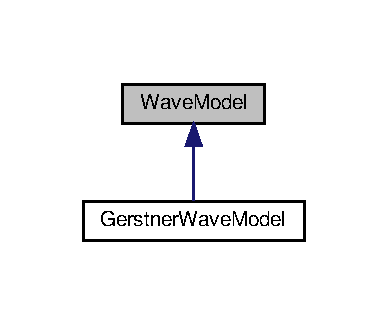
\includegraphics[width=186pt]{class_wave_model__inherit__graph}
\end{center}
\end{figure}
\subsection*{Fonctions membres publiques}
\begin{DoxyCompactItemize}
\item 
\mbox{\Hypertarget{class_wave_model_a22d9989890929f0418fcf7f1bd1fe489}\label{class_wave_model_a22d9989890929f0418fcf7f1bd1fe489}} 
{\bfseries Wave\+Model} (\hyperlink{class_wave_model}{Wave\+Model} \&\&model)
\item 
\mbox{\Hypertarget{class_wave_model_a1991dab09a570054adffc3677e218556}\label{class_wave_model_a1991dab09a570054adffc3677e218556}} 
{\bfseries Wave\+Model} (\hyperlink{class_wave_model}{Wave\+Model} const \&model)
\item 
\mbox{\Hypertarget{class_wave_model_a3b52480b59f4c5f3d0d749d400f9e14c}\label{class_wave_model_a3b52480b59f4c5f3d0d749d400f9e14c}} 
virtual \hyperlink{class_wave_model}{Wave\+Model} \& {\bfseries operator=} (\hyperlink{class_wave_model}{Wave\+Model} \&\&model)=0
\item 
\mbox{\Hypertarget{class_wave_model_a3794a5af00e6f216009fd8b54d48caf3}\label{class_wave_model_a3794a5af00e6f216009fd8b54d48caf3}} 
virtual \hyperlink{class_wave_model}{Wave\+Model} \& {\bfseries operator=} (\hyperlink{class_wave_model}{Wave\+Model} const \&model)=0
\item 
\mbox{\Hypertarget{class_wave_model_abe94f9621e5aaca300d8312479051710}\label{class_wave_model_abe94f9621e5aaca300d8312479051710}} 
virtual \hyperlink{class_dvector}{Dvector} $\ast$ {\bfseries get\+Wind\+Dir} ()
\item 
\mbox{\Hypertarget{class_wave_model_a829250f96303b3e9ddd9c2c6cbb0e3be}\label{class_wave_model_a829250f96303b3e9ddd9c2c6cbb0e3be}} 
virtual double {\bfseries get\+Average\+Matching} ()
\item 
\mbox{\Hypertarget{class_wave_model_ab72286fdfe57cebaae70af46c69dacb1}\label{class_wave_model_ab72286fdfe57cebaae70af46c69dacb1}} 
virtual double {\bfseries get\+Intensity} ()
\item 
\mbox{\Hypertarget{class_wave_model_af73c7bfe6c6c2d1546e7aaa966879ca3}\label{class_wave_model_af73c7bfe6c6c2d1546e7aaa966879ca3}} 
virtual double {\bfseries get\+Average\+Wave\+Length} ()
\item 
\mbox{\Hypertarget{class_wave_model_a6ce936ce9c4d27170bd0f7a6cd28b31f}\label{class_wave_model_a6ce936ce9c4d27170bd0f7a6cd28b31f}} 
virtual double {\bfseries get\+Ajust\+Wave\+Height} ()
\end{DoxyCompactItemize}


La documentation de cette classe a été générée à partir des fichiers suivants \+:\begin{DoxyCompactItemize}
\item 
/home/louis/\+Documents/2\+A/\+M\+P\+C/\+C\+P\+P/\+T\+P3\+\_\+sonoleta/headers/Wave\+Model.\+h\item 
/home/louis/\+Documents/2\+A/\+M\+P\+C/\+C\+P\+P/\+T\+P3\+\_\+sonoleta/src/Wave\+Model.\+cpp\end{DoxyCompactItemize}

\chapter{Documentation des fichiers}
\hypertarget{_dvector_8h}{}\section{Référence du fichier src/\+Dvector.h}
\label{_dvector_8h}\index{src/\+Dvector.\+h@{src/\+Dvector.\+h}}
{\ttfamily \#include $<$iostream$>$}\newline
Graphe des dépendances par inclusion de Dvector.\+h\+:
\nopagebreak
\begin{figure}[H]
\begin{center}
\leavevmode
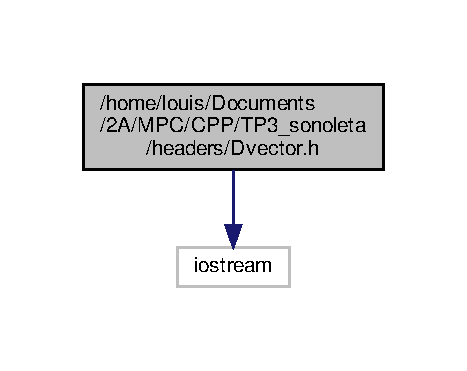
\includegraphics[width=156pt]{_dvector_8h__incl}
\end{center}
\end{figure}
\subsection*{Classes}
\begin{DoxyCompactItemize}
\item 
class \hyperlink{class_dvector}{Dvector}
\end{DoxyCompactItemize}


\subsection{Description détaillée}
classe vecteur de base, peut stocker des nombres au format double 
\hypertarget{_gerstner_wave_8h}{}\section{Référence du fichier /home/louis/\+Documents/2\+A/\+M\+P\+C/\+C\+P\+P/\+T\+P4\+\_\+sonoleta/headers/\+Gerstner\+Wave.h}
\label{_gerstner_wave_8h}\index{/home/louis/\+Documents/2\+A/\+M\+P\+C/\+C\+P\+P/\+T\+P4\+\_\+sonoleta/headers/\+Gerstner\+Wave.\+h@{/home/louis/\+Documents/2\+A/\+M\+P\+C/\+C\+P\+P/\+T\+P4\+\_\+sonoleta/headers/\+Gerstner\+Wave.\+h}}
{\ttfamily \#include \char`\"{}Complex\+Vector.\+h\char`\"{}}\newline
Graphe des dépendances par inclusion de Gerstner\+Wave.\+h\+:
\nopagebreak
\begin{figure}[H]
\begin{center}
\leavevmode
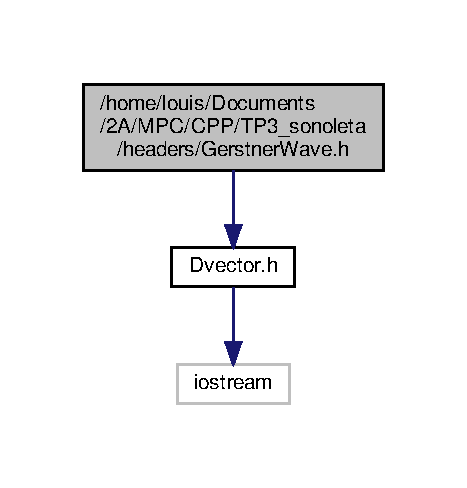
\includegraphics[width=350pt]{_gerstner_wave_8h__incl}
\end{center}
\end{figure}
Ce graphe montre quels fichiers incluent directement ou indirectement ce fichier \+:
\nopagebreak
\begin{figure}[H]
\begin{center}
\leavevmode
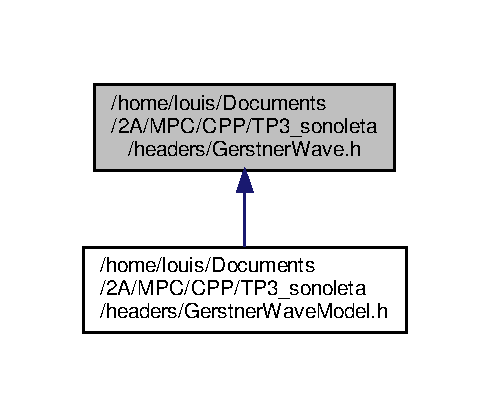
\includegraphics[width=350pt]{_gerstner_wave_8h__dep__incl}
\end{center}
\end{figure}
\subsection*{Classes}
\begin{DoxyCompactItemize}
\item 
class \hyperlink{class_gerstner_wave}{Gerstner\+Wave}
\end{DoxyCompactItemize}
\subsection*{Macros}
\begin{DoxyCompactItemize}
\item 
\mbox{\Hypertarget{_gerstner_wave_8h_a0b0fe599d70af5e8db73c78bc575bdb2}\label{_gerstner_wave_8h_a0b0fe599d70af5e8db73c78bc575bdb2}} 
\#define {\bfseries W\+\_\+\+T\+Y\+PE}~0
\end{DoxyCompactItemize}
\subsection*{Définitions de type}
\begin{DoxyCompactItemize}
\item 
\mbox{\Hypertarget{_gerstner_wave_8h_a8e9eb288b35318f759d070c21f86514c}\label{_gerstner_wave_8h_a8e9eb288b35318f759d070c21f86514c}} 
using {\bfseries Dvector} = \hyperlink{class_complex_vector}{Complex\+Vector}$<$ double $>$
\end{DoxyCompactItemize}
\subsection*{Fonctions}
\begin{DoxyCompactItemize}
\item 
double \hyperlink{_gerstner_wave_8h_aa6e95f4a08ffe3ce9c1086ba0e72dfca}{module} (\hyperlink{class_dvector}{Dvector} $\ast$dir)
\begin{DoxyCompactList}\small\item\em Calcule le module du vecteur d\textquotesingle{}onde. \end{DoxyCompactList}\item 
double \hyperlink{_gerstner_wave_8h_a9ec20622af66a127196b241dfb5f9416}{compute\+\_\+freq} (\hyperlink{class_dvector}{Dvector} $\ast$dir, int type=0, double D=0, double L=0, double T=1)
\begin{DoxyCompactList}\small\item\em Calcule la fréquence en fonction de la direction. \end{DoxyCompactList}\end{DoxyCompactItemize}


\subsection{Description détaillée}
classe des vague de Gerstner avec les méthodes associées 

\subsection{Documentation des fonctions}
\mbox{\Hypertarget{_gerstner_wave_8h_a9ec20622af66a127196b241dfb5f9416}\label{_gerstner_wave_8h_a9ec20622af66a127196b241dfb5f9416}} 
\index{Gerstner\+Wave.\+h@{Gerstner\+Wave.\+h}!compute\+\_\+freq@{compute\+\_\+freq}}
\index{compute\+\_\+freq@{compute\+\_\+freq}!Gerstner\+Wave.\+h@{Gerstner\+Wave.\+h}}
\subsubsection{\texorpdfstring{compute\+\_\+freq()}{compute\_freq()}}
{\footnotesize\ttfamily double compute\+\_\+freq (\begin{DoxyParamCaption}\item[{\hyperlink{class_dvector}{Dvector} $\ast$}]{dir,  }\item[{int}]{type,  }\item[{double}]{D,  }\item[{double}]{L,  }\item[{double}]{T }\end{DoxyParamCaption})}



Calcule la fréquence en fonction de la direction. 


\begin{DoxyParams}{Paramètres}
{\em dir} & \+: le vecteur d\textquotesingle{}onde \\
\hline
{\em type} & \+: le cas dans lequel on se trouve \textbackslash{} param D \+: distance du sol vis à vis du niveau moyen de l\textquotesingle{}océan \\
\hline
{\em T} & \+: période de répétition des vagues\\
\hline
\end{DoxyParams}
Renvoie la fréquence en fonction de plusieurs paramètres 
\begin{DoxyParams}{Paramètres}
{\em dir} & \+: vecteur d\textquotesingle{}ondes \\
\hline
{\em type} & \+: 0 \+: cas de la houle 1 \+: eau peu profonde 2 \+: avec la tension de surface 3 \+: Na\+Ni \\
\hline
{\em D} & \+: distance du sol au niveau moyen \\
\hline
{\em L} & \+: tension de surface (?) \\
\hline
{\em T} & \+: période de répétition des variations de hauteur \\
\hline
\end{DoxyParams}
\mbox{\Hypertarget{_gerstner_wave_8h_aa6e95f4a08ffe3ce9c1086ba0e72dfca}\label{_gerstner_wave_8h_aa6e95f4a08ffe3ce9c1086ba0e72dfca}} 
\index{Gerstner\+Wave.\+h@{Gerstner\+Wave.\+h}!module@{module}}
\index{module@{module}!Gerstner\+Wave.\+h@{Gerstner\+Wave.\+h}}
\subsubsection{\texorpdfstring{module()}{module()}}
{\footnotesize\ttfamily double module (\begin{DoxyParamCaption}\item[{\hyperlink{class_dvector}{Dvector} $\ast$}]{dir }\end{DoxyParamCaption})}



Calcule le module du vecteur d\textquotesingle{}onde. 


\begin{DoxyParams}{Paramètres}
{\em dir} & \+: le vecteur d\textquotesingle{}onde \\
\hline
\end{DoxyParams}

\hypertarget{_gerstner_wave_model_8h}{}\section{Référence du fichier /home/louis/\+Documents/2\+A/\+M\+P\+C/\+C\+P\+P/\+T\+P3\+\_\+sonoleta/headers/\+Gerstner\+Wave\+Model.h}
\label{_gerstner_wave_model_8h}\index{/home/louis/\+Documents/2\+A/\+M\+P\+C/\+C\+P\+P/\+T\+P3\+\_\+sonoleta/headers/\+Gerstner\+Wave\+Model.\+h@{/home/louis/\+Documents/2\+A/\+M\+P\+C/\+C\+P\+P/\+T\+P3\+\_\+sonoleta/headers/\+Gerstner\+Wave\+Model.\+h}}
{\ttfamily \#include \char`\"{}Dvector.\+h\char`\"{}}\newline
{\ttfamily \#include \char`\"{}Gerstner\+Wave.\+h\char`\"{}}\newline
{\ttfamily \#include \char`\"{}Wave\+Model.\+h\char`\"{}}\newline
Graphe des dépendances par inclusion de Gerstner\+Wave\+Model.\+h\+:
\nopagebreak
\begin{figure}[H]
\begin{center}
\leavevmode
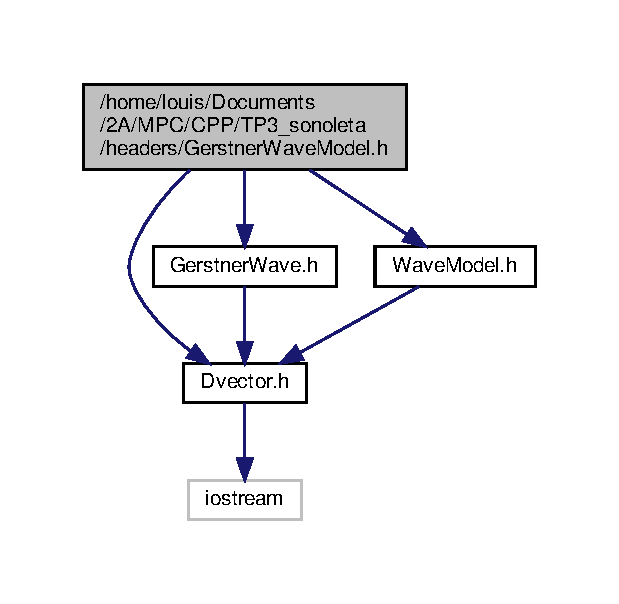
\includegraphics[width=297pt]{_gerstner_wave_model_8h__incl}
\end{center}
\end{figure}
\subsection*{Classes}
\begin{DoxyCompactItemize}
\item 
class \hyperlink{class_gerstner_wave_model}{Gerstner\+Wave\+Model}
\end{DoxyCompactItemize}


\subsection{Description détaillée}
Classe du modèle des vagues de Gerstner, sert à stocker une liste de vagues 
\hypertarget{_height_8h}{}\section{Référence du fichier /home/louis/\+Documents/2\+A/\+M\+P\+C/\+C\+P\+P/\+T\+P4\+\_\+sonoleta/headers/\+Height.h}
\label{_height_8h}\index{/home/louis/\+Documents/2\+A/\+M\+P\+C/\+C\+P\+P/\+T\+P4\+\_\+sonoleta/headers/\+Height.\+h@{/home/louis/\+Documents/2\+A/\+M\+P\+C/\+C\+P\+P/\+T\+P4\+\_\+sonoleta/headers/\+Height.\+h}}
\subsection*{Classes}
\begin{DoxyCompactItemize}
\item 
class \hyperlink{class_height}{Height}
\end{DoxyCompactItemize}


\subsection{Description détaillée}
Classe contenant l\textquotesingle{}ensemble des hauteurs dans un espace discrétisé 
%--- End generated contents ---

% Index
\backmatter
\newpage
\phantomsection
\clearemptydoublepage
\addcontentsline{toc}{chapter}{Index}
\printindex

\end{document}
